\documentclass[3p,11pt,fleqn,review,sort&compress]{elsarticle}
\bibliographystyle{elsarticle-num-names}
\usepackage{amsmath,amsfonts,amssymb,siunitx,float,subcaption,setspace,booktabs,diagbox,bm,tikz,structmech,mathtools,tikz-3dplot,pgfplots,gnuplot-lua-tikz,url,fontawesome5}
\usepackage{algorithm}
\usepackage{algpseudocode}
\usepackage{lineno}
\usepackage[many]{tcolorbox}
\usetikzlibrary{shapes.geometric}
\pgfplotsset{compat=1.8}
\journal{}
\newcommand*{\mb}[1]{\bm{#1}}
\newcommand*{\bbar}[1]{\bar{\bm{#1}}}
\newcommand*{\bhat}[1]{\hat{\bm{#1}}}
\newcommand*{\mT}{\mathrm{T}}
\newcommand*{\md}[1]{\mathrm{d}#1}
\newcommand*{\eqsref}[1]{Eq.~(\ref{#1})}
\newcommand*{\figref}[1]{Fig.~\ref{#1}}
\newcommand*{\tabref}[1]{Table~\ref{#1}}
\newcommand*{\algoref}[1]{Algorithm~\ref{#1}}
\newcommand*{\secref}[1]{\S~\ref{#1}}
\newcommand*{\diag}[1]{\text{diag}\left(#1\right)}
\newcommand*{\sign}[1]{\text{sign}\left(#1\right)}
\newcommand*{\dev}[1]{\text{dev}\left(#1\right)}
\newcommand*{\tr}[1]{\text{trace}\left(#1\right)}
\newcommand*{\ddfrac}[2]{\dfrac{\md{#1}}{\md{#2}}}
\newcommand*{\pdfrac}[2]{\dfrac{\partial{#1}}{\partial{#2}}}
\newcommand{\bsigma}{\mb{\sigma}}
\newcommand{\bvarepsilon}{\mb{\varepsilon}}
\newcommand{\beeta}{\mb{\eta}}
\newcommand{\bn}{\mb{n}}
\newcommand{\balpha}{\mb{\alpha}}
\newcommand{\bbeta}{\mb{\beta}}
\newcommand{\bgamma}{\mb{\gamma}}
\newcommand{\bq}{\mb{q}}
\newcommand{\bs}{\mb{s}}
\newcommand{\bc}{\mb{c}}
\newcommand{\be}{\mb{e}}
\newcommand{\bu}{\mb{u}}
\newcommand{\bv}{\mb{v}}
\newcommand{\bw}{\mb{w}}
\newcommand{\ba}{\mb{a}}
\newcommand{\bx}{\mb{x}}
\newcommand{\bbf}{\mb{f}}
\newdefinition{rmk}{Remark}
\DeclarePairedDelimiter\abs{\lvert}{\rvert}
\DeclarePairedDelimiter\norm{\lVert}{\rVert}
\tcbset{sharp corners,colback = white,before skip = 0.2cm,after skip = 0.5cm}
\newtcolorbox{Objective}{sharpish corners,boxrule = 0pt,leftrule = 4.5pt,enhanced,fuzzy shadow = {0pt}{-2pt}{-0.5pt}{0.5pt}{black!35}}
\makeatletter
\let\oldabs\abs
\def\abs{\@ifstar{\oldabs}{\oldabs*}}
\let\oldnorm\norm
\def\norm{\@ifstar{\oldnorm}{\oldnorm*}}
\newenvironment{breakablealgorithm}
{\begin{center}
\refstepcounter{algorithm}
\hrule height.8pt depth0pt \kern2pt
\renewcommand{\caption}[2][\relax]{
{\raggedright\textbf{\ALG@name~\thealgorithm} ##2\par}
\ifx\relax##1\relax
\addcontentsline{loa}{algorithm}{\protect\numberline{\thealgorithm}##2}
\else
\addcontentsline{loa}{algorithm}{\protect\numberline{\thealgorithm}##1}
\fi
\kern2pt\hrule\kern2pt
}}{\kern2pt\hrule\relax
\end{center}}
\begin{document}
\linenumbers
\begin{abstract}
\begin{linenumbers}
In this work, a fast algorithm to evaluate the dynamic response of nonviscously damped systems with arbitrary distributions of damping characterised by arbitrary kernel functions (both number and form) is proposed. The proposed algorithm requires mere level 2 BLAS operations. It can be integrated into existing analysis tools with various time integration methods in forms of either element-based dashpots or global damping model. Compared to other existing methods, the proposed algorithm shows superior accuracy while the corresponding computational cost is low.
\end{linenumbers}
\end{abstract}
\begin{keyword}
nonviscous damping\sep
direct integration\sep
arbitrary kernel
\end{keyword}
\begin{frontmatter}
\title{A Strategy for Fast Evaluation of Nonviscously Damped Systems With Arbitrary Kernels}
\author[add1]{Theodore~L.~Chang\corref{tlc}}\ead{tlcfem@gmail.com}
%\author[add2]{Chin-Long~Lee}
\cortext[tlc]{corresponding author}
\address[add1]{IRIS Adlershof, Humboldt-Universität zu Berlin, Berlin, Germany, 12489.}
%\address[add2]{Department of Civil and Natural Resources Engineering, University of Canterbury, Christchurch, New Zealand, 8041.}
\end{frontmatter}
\section{Introduction}
The equation of motion of nonviscously damped systems can be, conventionally, expressed as an integro-differential equation, namely, for elastic linear single degree of freedom systems,
\begin{gather}\label{eq:single_eom}
m\ddot{u}\left(t\right)+\left(g*\dot{u}\right)\left(t\right)+ku\left(t\right)=p\left(t\right),
\end{gather}
where $u(t)$ denotes the displacement, $\dot{(\cdot)}$ denotes time derivative, and $g=g(t)$ is the kernel function. Various forms have been proposed, see a brief summary by \citet[][Table 1.1]{Adhikari2014}.

The convolution term in \eqsref{eq:single_eom} can be expressed in integral form such that
\begin{gather}\label{eq:conv}
\left(g*\dot{u}\right)\left(t\right)=\int_0^tg\left(t-\tau\right)\dot{u}\left(\tau\right)\md{\tau}.
\end{gather}
Approaches to compute (or approximate, depending on one's perspective) it can be divided into two main categories:
\begin{enumerate}
\item Time Domain Methods\\
Since $g(t)$ is known, assume $\dot{u}(t)$ history is already obtained, \eqsref{eq:conv} can be numerically integrated for a given $t=T$ such that
\begin{gather}
\int_0^Tg\left(T-\tau\right)\dot{u}\left(\tau\right)\md{\tau}\approx\sum_i^n\omega_ig\left(T-t_i\right)\dot{u}\left(t_i\right),
\end{gather}
where $t_i=\left\{t_0,t_1,t_2,\cdots,t_n\right\}\in[0,T]$ that can be either evenly or unevenly spaced, and $\omega_i$ is the corresponding integration weight. If the exact $\dot{u}(t_i)$ is available, approximations (linear interpolation, weighted sum, etc.) based on adjacent known values are often adopted.
\item Frequency Domain Methods\\
\eqsref{eq:single_eom} can be equivalently expressed in the frequency domain via Laplace transform. For some kernels, analytical solutions can be found and converted back to the time domain.
\end{enumerate}
\section{Basics}
\subsection{Nonviscously Damped System}
Consider the equation of motion of a nonviscously damped inelastic multi-degree-of-freedom (MDOF) system,
\begin{gather}\label{eq:eom}
\mb{y}\left(\bu,\bv,\ba\right)+\bbf\left(t\right)=\mb{p}\left(t\right),
\end{gather}
where $\bu=\bu\left(t\right)$, $\bv=\bv\left(t\right)=\dot{\bu}$ and $\ba=\ba\left(t\right)=\dot{\bv}$ are the displacement, velocity and acceleration vectors, $\mb{y}=\mb{y}\left(\bu,\bv,\ba\right)$ is the resistance vector of the system, $\mb{p}=\mb{p}\left(t\right)$ is the external load vector, and $\bbf$ is the nonviscous damping force which can be expressed in the form of the convolution of the kernel $g=g\left(t\right)$ and the vector $\bw$, viz. $\bbf\left(t\right)=g*\bw$.

Note here, $\bw$ can be either the exact velocity vector $\bv$, or the subset of $\bv$ such that they share the same size but some velocity components in $\bv$ are replaced by zeros in $\bw$ on selected DoFs. This is beneficial when it comes to compositing flexible damping that will be discussed later in this work. Formally, it can be represented by
\begin{gather}
\bw=\mb{T}\bv,
\end{gather}
where $\mb{T}$ is a square diagonal matrix, the diagonal entries of which are either one or zero.

Since it is an inelastic system, the stiffness matrix $\mb{K}$, the viscous damping matrix $\mb{C}$ and the mass matrix $\mb{M}$ are
\begin{gather}
\pdfrac{\mb{y}}{\bu}=\mb{K},\qquad
\pdfrac{\mb{y}}{\bv}=\mb{C},\qquad
\pdfrac{\mb{y}}{\ba}=\mb{M}.
\end{gather}
The viscous damping matrix $\mb{C}$ may not be trivial as the system may consist of viscous damping components (e.g., viscous damper devices). Using $\bu$ as the basic quantity, the effective stiffness matrix $\bbar{K}$
\begin{gather}
\bbar{K}=\ddfrac{\mb{y}}{\bu}=\mb{K}+\mb{C}\ddfrac{\bv}{\bu}+\mb{M}\ddfrac{\ba}{\bu}
\end{gather}
is the combination of the three, its specific form depends on the specific time integration method used.
\section{Nonviscous Damping With A Single Exponential Kernel}
\subsection{A Single Exponential Kernel}
We start with the scalar-valued exponential kernel function
\begin{gather}
g=g\left(t\right)=m\exp\left(-st\right),
\end{gather}
where $s$ is often denoted by the relaxation parameter $\mu$, $m$ is often denoted by $c\mu$ in which $c$ is the damping constant. In this work, $s$ and $m$ are adopted for brevity.
The convolution can be then expressed as
\begin{gather}\label{eq:single_conv}
\bbf\left(t\right)=g*\bw=\int_0^tg(t-\tau)\cdot\bw\left(\tau\right)~\md{\tau}=\int_0^tm\exp\left(-s\left(t-\tau\right)\right)\cdot\bw\left(\tau\right)~\md{\tau}.
\end{gather}
\eqsref{eq:single_conv} corresponds to the solution of the following ODE \citep[see, e.g.,][\S~80]{Zwillinger2021},
\begin{gather}\label{eq:single_conv_ode}
\bbf'=-s\bbf+m\bw.
\end{gather}
It can be validated by solving \eqsref{eq:single_conv_ode} with the assist of the integrating factor $\exp\left(st\right)$.
\subsection{An Efficient Algorithm}
Instead of directly integrating \eqsref{eq:single_conv} using higher-order methods (such as the Runge--Kutta family), \eqsref{eq:single_conv_ode} can be combined with \eqsref{eq:eom} to develop an efficient algorithm.

Given that popular time integration methods are of second order accuracy, in the context of a discretised iterative solving schema, \eqsref{eq:single_conv_ode} can be rewritten as follows using Heun's method, which is second order accurate, accordingly,
\begin{gather}
\tilde{\bbf}_{n+1}=\bbf_n+\Delta{}t\left(-s\bbf_n+m\bw_n\right),\\
\bbf_{n+1}=\bbf_n+\dfrac{\Delta{}t}{2}\left(-s\bbf_n+m\bw_n-s\tilde{\bbf}_{n+1}+m\bw_{n+1}\right).
\end{gather}
Expanding and rearranging lead to
\begin{gather}
\bbf_{n+1}=
\left(1-s\Delta{}t+\dfrac{s^2\Delta{}t^2}{2}\right)\bbf_n
+\dfrac{m\Delta{}t}{2}\left(1-s\Delta{}t\right)\bw_n
+\dfrac{m\Delta{}t}{2}\bw_{n+1}.
\end{gather}

In the context of a discretised iterative solving scheme, \eqsref{eq:single_conv_ode} can be rewritten as follows using the backward (implicit) Euler method,
\begin{gather}\label{eq:discretised_a}
\dfrac{\bbf_{n+1}-\bbf_n}{\Delta{}t}=-s\bbf_{n+1}+m\bw_{n+1},
\end{gather}
in which subscripts $\left(\cdot\right)_{n+1}$ and $\left(\cdot\right)_n$ denote the corresponding quantity at $t_n$ and $t_{n+1}=t_n+\Delta{}t$.
Rearranging \eqsref{eq:discretised_a} yields
\begin{gather}\label{eq:discretised_b}
\left(1+s\Delta{}t\right)\bbf_{n+1}-\bbf_n-m\Delta{}t\bw_{n+1},
\end{gather}
thus
\begin{gather}\label{eq:discretised_c}
\bbf_{n+1}=\dfrac{1}{1+s\Delta{}t}\bbf_n+\dfrac{m\Delta{}t}{1+s\Delta{}t}\bw_{n+1}.
\end{gather}

It must be pointed out that the idea to introduce an internal variable is similar to the approach presented by \citet[][see \S~4.3]{Adhikari2014}. In this work, instead of the filtered velocity \citep[][see Eq. 4.23]{Adhikari2014}, the nonviscous damping force is chosen as the internal variable, which, as can be seen later, eventually leads to a system that can be effectively solved.

Assuming \eqsref{eq:eom} is satisfied at $t_{n+1}$\footnote{This assumption is not always valid as some time integration methods establish the EOM elsewhere, see, for example, the generalised-$\alpha$ method, the GSSSS method, the Bathe two-step method, the OALTS method, etc.}, then, accounting for \eqsref{eq:discretised_c}, \eqsref{eq:eom} (with the subscript $\left(\cdot\right)_{n+1}$ dropped for brevity) is
\begin{gather}\label{eq:residual}
\mb{y}+\dfrac{1}{1+s\Delta{}t}\bbf_n+\dfrac{m\Delta{}t}{1+s\Delta{}t}\bw=\mb{p}.
\end{gather}
Differentiation leads to the following revised effective stiffness $\bhat{K}$,
\begin{gather}\label{eq:revised_k}
\bhat{K}=\bbar{K}+\dfrac{m\Delta{}t}{1+s\Delta{}t}\mb{T}\ddfrac{\bv}{\bu}.
\end{gather}
Typically, $\ddfrac{\bv}{\bu}$ reduces to a scalar constant (multiplied by an identity matrix), for example, in the Newmark method, it is $\dfrac{\gamma}{\beta\Delta{}t}$.

By introducing the revised resistance $\bhat{y}$ as
\begin{gather}\label{eq:revised_y}
\bhat{y}=\mb{y}+\dfrac{1}{1+s\Delta{}t}\bbf_n+\dfrac{m\Delta{}t}{1+s\Delta{}t}\bw,
\end{gather}
the final system to be solved is
\begin{gather}\label{eq:revised_system}
\bhat{K}\delta\bu=\mb{q}-\bhat{y}.
\end{gather}

The local iteration body is summarised in \algoref{algo:single_model}.
\begin{breakablealgorithm}
\setstretch{1.8}
\caption{iteration body of solving nonviscously damped system with one exponential kernel}\label{algo:single_model}
\begin{algorithmic}
\State \textbf{Input}: $\bbar{K}$, $\bu$, $\bv$, $\mb{y}$, $\mb{p}$ (quantities obtained via conventional manner as if there is no nonviscous damping) and $\bbf_n$
\State \textbf{Output}: $\bu$
\State compute $\bw$ from $\bv$
\State \faMicrochip~compute revised stiffness $\bhat{K}=\bbar{K}+\dfrac{m\Delta{}t}{1+s\Delta{}t}\mb{T}\ddfrac{\bv}{\bu}$\Comment{\eqsref{eq:revised_k}}
\State \faMicrochip~compute revised resistance $\bhat{y}=\mb{y}+\dfrac{1}{1+s\Delta{}t}\bbf_n+\dfrac{m\Delta{}t}{1+s\Delta{}t}\bw$\Comment{\eqsref{eq:revised_y}}
\State $\delta\bu=\bhat{K}^{-1}\left(\mb{p}-\bhat{y}\right)$\Comment{\eqsref{eq:revised_system}}
\State update and return $\bu\leftarrow\bu+\delta\bu$
\end{algorithmic}
\end{breakablealgorithm}
The steps with a leading \faMicrochip~symbol augment global effective stiffness and resistance to obtain $\bhat{K}$ and $\bhat{y}$. Those are additional steps that need to be computed compared to a conventional algorithm for nonviscously damped systems. Once convergence is achieved, it is necessary to store the history of nonviscous damping force $\bbf_n\leftarrow\bbf$.

Unlike other algorithms, such as the one by \citet{Cortes2009}, \algoref{algo:single_model} does not impose additional requirements to the time integration method used.
\subsection{Complexity Analysis}
The term $\mb{T}\ddfrac{\bv}{\bu}\delta\bu$ can be efficiently computed by masking $\delta\bu$ as $\mb{T}$ is a diagonal matrix while $\ddfrac{\bv}{\bu}$ can be equivalently converted into a scalar (see discussion before). Assuming the system has a size of $n$, it requires at most $n$ floating point number arithmetic. All three extra steps require pure vector operations, the total number of floating point number multiplications is $6n$, that is a time complexity of $\mathcal{O}\left(n\right)$.

\algoref{algo:single_model} requires no memory reallocation, the additional storage needed is for the nonviscous damping forces $f_n$, implying a space complexity of $\mathcal{O}\left(n\right)$.
\section{Nonviscous Damping With Arbitrary Kernel}
\subsection{Sum of Exponentials}
Now consider, instead of a single exponential function, multiple exponential functions such that
\begin{gather}\label{eq:sum_exp}
g=\sum_{l=1}^{j}g_l\left(t\right)=\sum_{l=1}^{j}m_l\exp\left(-s_lt\right),
\end{gather}
where $m_l$ and $s_l$ can be complex numbers, then
\begin{gather}\label{eq:sum_conv}
\bbf\left(t\right)=g*\bw=\sum_{l=1}^{j}g_l\left(t\right)*\bw=\sum_{l=1}^{j}\bbf_l.
\end{gather}
For each of $\bbf_l$, \eqsref{eq:discretised_b} also holds and only involves $\bbf_l$ itself and the common quantity $\bw$. Thus,
\begin{gather}
\bbf_l=\dfrac{1}{1+s_l\Delta{}t}\bbf_{l,n}+\dfrac{m_l\Delta{}t}{1+s_l\Delta{}t}\bw.
\end{gather}

Similar to the single function case, substituting $\bbf_l$ into \eqsref{eq:eom}, differentiation yields the revised stiffness
\begin{gather}\label{eq:revised_k_multi}
\bhat{K}=\bbar{K}+\sum_{l=1}^{j}\dfrac{m_l\Delta{}t}{1+s_l\Delta{}t}\mb{T}\ddfrac{\bv}{\bu},
\end{gather}
and the revised resistance
\begin{gather}\label{eq:revised_y_multi}
\bhat{y}=\mb{y}+\sum_{l=1}^{j}\dfrac{1}{1+s_l\Delta{}t}\bbf_{l,n}+\sum_{l=1}^{j}\dfrac{m_l\Delta{}t}{1+s_l\Delta{}t}\bw.
\end{gather}

Noting that within each sum, the operations performed are identical to that in the single function case, the complexity in this case is $\mathcal{O}\left(jn\right)$ for both time and space.
\subsection{Arbitrary Kernel}
\citet{Gao2022} presented a method to approximate a given arbitrary function $g\left(t\right)$ with arbitrary accuracy within a given interval, using multiple exponential functions, that is
\begin{gather}
\max_{t\in{}I}{\abs{g\left(t\right)-\sum_jm_j\exp\left(-s_jt\right)}}<\epsilon,
\end{gather}
where $I$ is a finite interval that could be an arbitrary subset of $\mathbb{R}^+$, $\epsilon$ is the error tolerance.

By assigning a tolerance close to (or less than) the machine error, an accurate equivalence of arbitrary kernel function can be obtained for nonviscous damping computation. In practice, such a tolerance only needs to be smaller than analysis tolerance.
\subsection{Composition of Damping}
It is possible to further assign multiple arbitrary kernels to different subsets of velocity vector. Formally,
\begin{gather}
\bbf=\sum_{k=1}^{i}g^k\bw^k,
\end{gather}
where $g^k$ is the arbitrary kernel applied to $\bw^k$,
\begin{gather}
g^k=\sum_{l=1}^{j^k}g_l^k\left(t\right)=\sum_{l=1}^{j^k}m_l^k\exp\left(-s_l^kt\right),
\end{gather}
in its explicit form
\begin{gather}\label{eq:composition}
\bbf=\sum_{k=1}^{i}\sum_{l=1}^{j^k}\bbf_l^k=\sum_{k=1}^{i}\sum_{l=1}^{j^k}g_l^k\left(t\right)\bw^k=\sum_{k=1}^{i}\sum_{l=1}^{j^k}m_l^k\exp\left(-s_l^kt\right)\bw^k.
\end{gather}

Since additivity still holds, there is no essential difference between \eqsref{eq:sum_exp} and \eqsref{eq:composition}. $m_l^k$ and $s_l^k$ are parameters for $l$-th component of $k$-th kernel. $\bw^k=\mb{T}^k\bv$ can be obtained by either node-based or element-based rules. For the former, it is assumed different regions (characterised by nodes) possess different damping response. For the latter, it is assumed different elements possess different damping response, similar to a typical assembly process. No matter how $\bw^k$ is constructed, the revised stiffness and resistance for each $\bbf_l^k$ only require vector--scalar operation.

Denoting
\begin{gather}
j^\text{max}=\max_{k\in\{1,2,\cdots,i\}}\left(j^k\right),
\end{gather}
the time and space complexity is $\mathcal{O}\left(ij^\text{max}n\right)$.

\section{Numerical Examples}
\subsection{SDOF System With Single Exponential}
We start with the validation of \algoref{algo:single_model}. To this end, consider the free vibration of a SDOF system with one exponential kernel such that the EOM can be expressed as
\begin{gather}
m\ddot{u}\left(t\right)+\int_0^tc\mu\exp\left(-\mu\left(t-\tau\right)\right)\dot{u}\left(\tau\right)\md{\tau}+ku\left(t\right)=0.
\end{gather}
The parameters are set to $m=1$, $c=2$, $\mu=1$, $k=100$.
The initial conditions are $u\left(0\right)=1$, $\dot{u}\left(0\right)=1$ and $\ddot{u}\left(0\right)=1$.
The closed form solution can be found in \secref{sec:analytical_sdof}.
The Newmark (constant acceleration) method is used for time integration.
The displacement history and the corresponding error convergence are shown in \figref{fig:sdof}.

The maximum of the difference between numerical and analytical solutions is taken as the absolute error $\epsilon$. It is evident that \eqsref{eq:discretised_c} retains the second-order accuracy of the Newmark method.
\begin{figure}[H]
\centering
\includegraphics{PY/single_exp}
\caption{displacement history and error analysis of SDOF oscillator with one exponential kernel}\label{fig:sdof}
\end{figure}
\subsection{Three DOF System}
\begin{figure}[H]
\centering
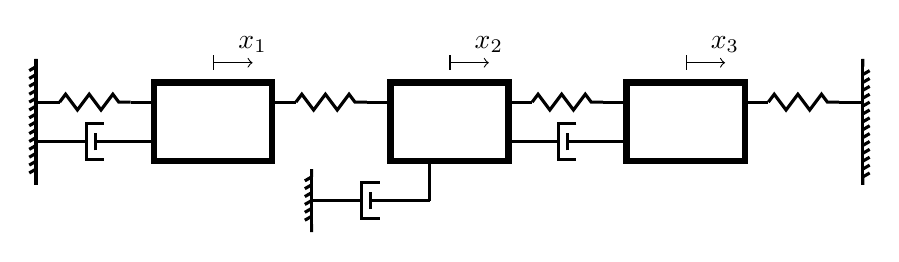
\begin{tikzpicture}
\draw[line width=.8mm](2,0)rectangle++(1.5,1);
\draw[line width=.8mm](5,0)rectangle++(1.5,1);
\draw[line width=.8mm](8,0)rectangle++(1.5,1);
\setstructmech{linewidth=.4mm}
\Spring{.5,.75}{2,.75}{1.5}
\Spring{3.5,.75}{5,.75}{1.5}
\Spring{6.5,.75}{8,.75}{1.5}
\Spring{9.5,.75}{11,.75}{1.5}
\Dashpot{6.5,.25}{8,.25}{1.5}
\Dashpot{.5,.25}{2,.25}{1.5}
\Dashpot{4,-.5}{5.5,-.5}{1.5}
\FixedSupport[-90]{.5,.5}{2}
\FixedSupport[90]{11,.5}{2}
\FixedSupport[-90]{4,-.5}
\draw[line width=.4mm](5.5,-.5)--++(0,.5);
\draw[|->](2.75,1.25)--++(.5,0)node[above]{$x_1$};
\draw[|->](5.75,1.25)--++(.5,0)node[above]{$x_2$};
\draw[|->](8.75,1.25)--++(.5,0)node[above]{$x_3$};
\end{tikzpicture}
\end{figure}

\begin{figure}[H]
\centering
\includegraphics{PY/three_dof}
\caption{displacement history and error analysis of three DOF system with two exponential kernels}\label{fig:three}
\end{figure}

The analytical solution is obtained via modal analysis/expansion, the relevant derivations can be seen elsewhere \citep[see][\S~4.6.2]{Adhikari2014}.

Compared to the numerical solutions (with $\Delta{}t=\SI{0.05}{\second}$) obtained by \citet{Cortes2009}, the present algorithm yields more accurate results. Even for a large time step $\Delta{}t=\SI{0.1}{\second}$, unlike other methods \citep{Liu2023}, there is no severe deviation observed.

The convergence of absolute error again shows a quadratic order, implying the simple \eqsref{eq:eqv_sys} is effective.
\section{Conclusions}
In this work, a performant general--purpose algorithm integrating nonviscous damping with direct time integration methods with arbitrary kernel functions is proposed.
The proposed algorithm solves the nonviscously damped dynamic systems directly in the time domain and uses the VPMR algorithm to approximate arbitrary kernels.
The proposed algorithm can be implemented as either a global damping model or element style nonviscous dashpot, it minimises the computational cost with superior accuracy and can be integrated with various direct time integration methods.

\add{The proposed algorithm offers an alternative tool to perform numerical analyses. However, in terms of identification and quantification of nonviscous damping, numerical results shall be validated against real structure data, and this is recommended for future research.}

An open source port of the VPMR algorithm is available online\footnote{https://github.com/TLCFEM/vpmr}.
The nonviscous damping has been implemented in \texttt{suanPan} \citep{Chang2023} as both a dashpot element and a global damping model. All numerical models and the corresponding analytical solutions (if applicable) are available in this repository\footnote{https://github.com/TLCFEM/nonviscous-implementation}.
\appendix
\section{Closed Form Solution}\label{sec:analytical_sdof}
Performing Laplace transform of the following homogeneous ODE
\begin{gather}\label{eq:single_exp}
m\ddot{u}\left(t\right)+\int_0^tc\mu\exp\left(-\mu\left(t-\tau\right)\right)\dot{u}\left(\tau\right)\md{\tau}+ku\left(t\right)=0
\end{gather}
yields
\begin{gather}
m\left(s^2U-su_0-\dot{u}_0\right)
+c\mu\dfrac{sU-u_0}{s+\mu}
+kU
=0,
\end{gather}
where $U=U\left(s\right)$. Rearranging gives
\begin{gather}
\left(
s^3
+\mu{}s^2
+\dfrac{c\mu+k}{m}s
+\dfrac{k\mu}{m}\right)U
=
u_0s^2
+\left(\mu{}u_0+\dot{u}_0\right)s
+\dfrac{c\mu{}}{m}u_0
+\mu\dot{u}_0.
\end{gather}
Assuming the three roots of the characteristic equation are $r_1$, $r_2$ and $r_3$, and $U$ can be expressed as
\begin{gather}
U\left(s\right)=\sum_{i=1}^3\dfrac{P_i}{s-r_i},
\end{gather}
expanding and comparing,
\begin{gather}
\begin{bmatrix}
1&1&1\\
-r_2-r_3&-r_1-r_3&-r_1-r_2\\
r_2r_3&r_1r_3&r_1r_2
\end{bmatrix}
\begin{bmatrix}
P_1\\P_2\\P_3
\end{bmatrix}
=
\begin{bmatrix}
u_0\\
\mu{}u_0+\dot{u}_0\\
\dfrac{c\mu{}}{m}u_0
+\mu\dot{u}_0
\end{bmatrix}.
\end{gather}
After solving $P_i$, transforming $U$ back to the time domain gives the solution
\begin{gather}
u(t)=\sum_{i=1}^3P_i\exp\left(r_it\right).
\end{gather}
\section{VPMR Approximation of Gaussian Kernels}\label{sec:vpmr}
For kernel
\begin{gather}
g_1=1.2\sqrt{\dfrac{1}{\pi}}\exp\left(-t^2\right),
\end{gather}
the following $m_l$ and $s_l$ are used.
\begin{table}[H]
\centering\scriptsize
\caption{$m_l$ and $s_l$ of the approximation of kernel $g(t)=1.2\sqrt{1/\pi}\exp(-t^2)$}\label{tab:vpmr_g1}
\begin{tabular}{r|r|r|r}
    \toprule
                      $\Re(m_l)$ &                   $\Im(m_l)$ &                  $\Re(s_l)$ &                   $\Im(s_l)$ \\ \midrule
     \num{3.140856464484043e+01} &                              & \num{4.501691936620960e+00} &                              \\
    \num{-1.670698314099744e+01} &  \num{1.694493634189165e+01} & \num{4.495083727260961e+00} &  \num{1.039544182084329e+00} \\
    \num{-1.670698314099744e+01} & \num{-1.694493634189165e+01} & \num{4.495083727260961e+00} & \num{-1.039544182084329e+00} \\
     \num{4.311759374683535e-03} &  \num{1.018262051173052e+01} & \num{4.474910170433406e+00} & \num{-2.094934226610453e+00} \\
     \num{4.311759374683535e-03} & \num{-1.018262051173052e+01} & \num{4.474910170433406e+00} &  \num{2.094934226610453e+00} \\
     \num{1.580121702525763e+00} &  \num{1.715134770620785e+00} & \num{4.440014388559026e+00} &  \num{3.185164080597838e+00} \\
     \num{1.580121702525763e+00} & \num{-1.715134770620785e+00} & \num{4.440014388559026e+00} & \num{-3.185164080597838e+00} \\
    \num{-2.528351542418222e-01} &  \num{3.658045212954592e-02} & \num{4.387994146629901e+00} & \num{-4.337651474857473e+00} \\
    \num{-2.528351542418222e-01} & \num{-3.658045212954592e-02} & \num{4.387994146629901e+00} &  \num{4.337651474857473e+00} \\
     \num{9.686449948037756e-03} &  \num{4.313057282514074e-03} & \num{4.313868192979954e+00} & \num{-5.601534417677513e+00} \\
     \num{9.686449948037756e-03} & \num{-4.313057282514074e-03} & \num{4.313868192979954e+00} &  \num{5.601534417677513e+00} \\
    \num{-7.018890017962145e-05} &  \num{5.918104645530206e-05} & \num{4.204602737864920e+00} &  \num{7.100600444858869e+00} \\
    \num{-7.018890017962145e-05} & \num{-5.918104645530206e-05} & \num{4.204602737864920e+00} & \num{-7.100600444858869e+00} \\ \bottomrule
\end{tabular}
\end{table}
For kernel
\begin{gather}
g_2=0.4\sqrt{\dfrac{5}{\pi}}\exp\left(-5t^2\right),
\end{gather}
the following $m_l$ and $s_l$ are used.
\begin{table}[H]
\centering\tiny
\caption{$m_l$ and $s_l$ of the approximation of kernel $g(t)=0.4\sqrt{5/\pi}\exp(-5t^2)$}\label{tab:vpmr_g2}
\begin{tabular}{r|r|r|r}
    \toprule
                      $\Re(m_l)$ &                   $\Im(m_l)$ &                  $\Re(s_l)$ &                   $\Im(s_l)$ \\ \midrule
     \num{2.390615900072754e+01} &                              & \num{1.008763774835104e+01} &                              \\
    \num{-1.276225642689750e+01} &  \num{1.286047649037308e+01} & \num{1.007282883037510e+01} &  \num{2.322701258992829e+00} \\
    \num{-1.276225642689750e+01} & \num{-1.286047649037308e+01} & \num{1.007282883037510e+01} & \num{-2.322701258992829e+00} \\
     \num{5.321829762994009e-02} &  \num{7.760888995593035e+00} & \num{1.002759753347236e+01} & \num{-4.680737620510257e+00} \\
     \num{5.321829762994009e-02} & \num{-7.760888995593035e+00} & \num{1.002759753347236e+01} &  \num{4.680737620510257e+00} \\
     \num{1.194094646597810e+00} &  \num{1.321100573765225e+00} & \num{9.949275285221848e+00} &  \num{7.116484734939028e+00} \\
     \num{1.194094646597810e+00} & \num{-1.321100573765225e+00} & \num{9.949275285221848e+00} & \num{-7.116484734939028e+00} \\
    \num{-1.932626856086916e-01} &  \num{3.038377981850687e-02} & \num{9.832324567288200e+00} & \num{-9.691168168166810e+00} \\
    \num{-1.932626856086916e-01} & \num{-3.038377981850687e-02} & \num{9.832324567288200e+00} &  \num{9.691168168166810e+00} \\
     \num{7.494857745336815e-03} &  \num{3.209850541294188e-03} & \num{9.665305732814788e+00} & \num{-1.251463324996230e+01} \\
     \num{7.494857745336815e-03} & \num{-3.209850541294188e-03} & \num{9.665305732814788e+00} &  \num{1.251463324996230e+01} \\
    \num{-5.493762818993658e-05} &  \num{4.496057010788951e-05} & \num{9.418507257498408e+00} &  \num{1.586378248808019e+01} \\
    \num{-5.493762818993658e-05} & \num{-4.496057010788951e-05} & \num{9.418507257498408e+00} & \num{-1.586378248808019e+01} \\ \bottomrule
\end{tabular}
\end{table}
%Using the following parameters:
%        nc = 4.
%         n = 40.
%     order = 800.
% precision = 684.
% tolerance = 1.0000e-12.
%    kernel = 1.2*sqrt(1/pi)*exp(-t^2).


%Using the following parameters:
%        nc = 4.
%         n = 60.
%     order = 800.
% precision = 1044.
% tolerance = 1.0000e-13.
%    kernel = .4*sqrt(5/pi)*exp(-5*t^2).


\bibliography{BIB}
\end{document}